\documentclass[11pt]{article}

\usepackage[utf8]{inputenc}
\usepackage[margin=1in]{geometry}
\usepackage{titlesec}
\usepackage{enumitem}
\usepackage{hyperref}
\usepackage{tikz}
\usetikzlibrary{positioning}
\usepackage{amsmath, amssymb}

\begin{document}

\begin{titlepage}
\centering
\vspace*{2cm}
{\normalsize INSuRE Fall 2026\\Project Proposal - 09/09/2026\par}
\vspace{1cm}
{\Huge\bfseries Cryptographic Protocol Analysis and Verification\par}
\vspace{25em}
Investigators:\par
\vspace{0.4cm}
\textbf{The University of Texas at Dallas}\par
William T. Doan - doan@utdallas.edu\par
Aendri Singh - aendri.singh@utdallas.edu\par
Pooya Zolfagharkhani - pooya.zolfagharkhani@utdallas.edu\par
Andrew Bourinski - andrew.bourinski@utdallas.edu\par
Brian Ricks - absolutefunk@utdallas.edu\par
\vspace{0.7cm}
Problem Mentor(s):\par
\vspace{0.4cm}
\textbf{The National Security Agency of the United States}\par
Edward Ziegler\par
\vfill
\end{titlepage}

\tableofcontents
\newpage

\section{Project Summary} 

\subsection{Top Level Research Project Description}
Cryptographic protocols are fundamental to secure distributed communications across the world, yet informal design practices and unexpressed assumptions often leave protocols open to attack. As such, protocols must undergo rigorous testing and verification to ensure that they remain secure in all circumstances. This research investigates methods to improve cryptographic protocol verification by comparing Cryptographic Protocol Shapes Analyzer (CPSA) and s(CASP), focusing on each framework's ability to detect protocol vulnerabilities that the other overlooks. While CPSA analyzes protocols by characterizing all possible execution shapes, s(CASP) utilizes goal oriented constraint answer set programming to provide verifiable, step by step traces of protocol execution paths. By benchmarking each framework's ability to identify both documented and novel protocol vulnerabilities, this work will assess their respective capabilities, trade offs, and limitations. In addition to this verification, this research will also explore whether active automata learning can expose vulnerabilities that static methods miss. If we treat an algorithm as a black box, we can use the $L^*$ algorithm to learn and construct an equivalent representation of the algorithm through carefully created input queries and their observed outputs. By probing the learned model, we will determine if CPSA and s(CASP) missed any vulnerabilities or attack vectors.\\

\noindent
\textit{Keywords—}Answer Set Programming, s(ASP), s(CASP), Cryptographic Protocol Analysis,\\Backward-Chaining, CPSA, Strand Spaces, Dolev-Yao Model, BAN Logic, Model Checking, Theorem Proving, Active Automata Learning, $L^*$ Algorithm, Deterministic Finite Automata, Machine Learning, Large Language Models, Model Context Protocol, TLS, OAuth, Prompt Injection, Maude-NPA, Tamarin Prover, ProVerif, Cryptol, Formal Verification, Domain Specific Language

\subsection{Terminology}
\begin{itemize}
    \item \textbf{Cryptographic Protocol}: A distributed algorithm that describes precisely the interactions between two or more entities in service of agreed security objectives \cite{toorani2016securityprotocolsnutshell}.
    \item \textbf{Answer Set Programming (ASP)}: A modeling language that states a computational problem in terms of constraints over a binary domain \cite{10.1145/2043174.2043195}.
    \item \textbf{Atom}: An elementary proposition that makes up a literal \cite{10.1145/2043174.2043195}.
    \item \textbf{Literal}: An atom or its negation \cite{10.1145/2043174.2043195}.
    \item \textbf{Rule}: A justification of the form $a \leftarrow b_1,\dots, b_m, not\ c_1,\dots,not\ c_n$, where the head $a$ is derived by a body of literals that all resolve to true \cite{10.1145/2043174.2043195}.
    \item \textbf{Program}: A finite collection of rules \cite{10.1145/2043174.2043195}.
    \item \textbf{Fact}: A rule with no body, i.e., no preconditions, and is therefore established directly \cite{10.1145/2043174.2043195}.
    \item \textbf{Answer Set}: The formalization of a rule's intuition as exactly the derivations of each sub-rule within it \cite{10.1145/2043174.2043195}.
    \item \textbf{Grounded Program}: A program containing no variables \cite{10.1145/2043174.2043195}.
    \item \textbf{Grounding}: The process by which variables and recursive rule invocations are removed from a program \cite{10.1145/2043174.2043195}.
    \item \textbf{s(ASP)}: A goal-directed, predicate-level form of ASP that circumvents grounding entirely, avoiding exponential growth in program size \cite{Marple2017TheS}.
    \item \textbf{s(CASP)}: An extension of s(ASP) to variables over continuous domains, treating them as constraints on the answer rather than requiring grounding and resolution \cite{ARIAS_CARRO_SALAZAR_MARPLE_GUPTA_2018}.
    \item \textbf{Backward-Chaining}: The query process of s(CASP) in which evaluation begins at the goal and works backwards through rule heads to their bodies, generating subgoals until the proof chain terminates at facts \cite{Arias_2020}.
    \item \textbf{Trace}: The record of the backward-chaining process that makes s(CASP) explainable \cite{Arias_2020}.
    \item \textbf{CPSA (Cryptographic Protocol Shapes Analyzer)}: A tool that attempts to enumerate all unique executions, or shapes, of a protocol that are possible.
    \item \textbf{Shape}: A unique, possible execution of a cryptographic protocol, as enumerated by CPSA.
    \item \textbf{Dolev-Yao Model}: A model of network communication granting the adversary complete control over messages sent between principals, within which CPSA enumerates protocol shapes \cite{1056650}.
    \item \textbf{Formal Verification}: The use of tools and techniques to mathematically verify the security properties of a cryptographic protocol specification against a well-defined set of assumptions.
    \item \textbf{Strand}: A sequence of events representing either an execution by a legitimate party or a sequence of a perpetrator's actions \cite{doi:10.3233/JCS-1999-72-304}.
    \item \textbf{Burrows-Abadi-Needham (BAN) Logic}: A belief logic that analyzes an information exchange protocol by determining whether the information it trades is trustworthy, protected against eavesdropping, or both \cite{10.1145/77648.77649}.
    \item \textbf{Model Checking}: One of the two techniques, alongside theorem proving, that dominate the formal verification of security protocols \cite{pourpouneh}.
    \item \textbf{Theorem Proving}: The verification technique, complementary to model checking, that derives a protocol's correctness from a deduction system \cite{pourpouneh}.
    \item \textbf{Regular Language}: The class of languages that Angluin's $L^*$ algorithm is capable of learning \cite{angluin1987}.
    \item \textbf{Minimally Adequate Teacher (MAT)}: An oracle, assumed by $L^*$, capable of answering membership and equivalence queries about an unknown regular language \cite{angluin1987}.
    \item \textbf{Membership Query}: A query to the Minimally Adequate Teacher asking whether a given string belongs to the unknown target language \cite{angluin1987}.
    \item \textbf{Equivalence Query}: A query to the Minimally Adequate Teacher asking whether a hypothesized language equals the unknown target language, returning a counterexample when it does not \cite{angluin1987}.
    \item \textbf{$L^*$ Algorithm}: An algorithm, introduced by Angluin, that identifies an unknown regular set using only membership and equivalence queries to a Minimally Adequate Teacher \cite{angluin1987}.
    \item \textbf{Deterministic Finite Automaton (DFA)}: The model of computation that de Ruiter observed typically underlies the implementation of security protocols \cite{deruiter2015}.
    \item \textbf{Active Automata Learning}: The class of techniques, exemplified by $L^*$, that infer an automaton describing a black-box system's behavior through targeted queries \cite{deruiter2015}.
\end{itemize}

\subsection{Team Member Responsibilities}
All team members will be responsible for keeping abreast with the development, progress, and final delivery of this project in addition to any research, coding, implementation, testing, and presentation responsibilities thereof. Below are the particular responsibilities expected of each member on top of the general team citizenship responsibilities aforementioned.  \\

\noindent
\textbf{William T. Doan} will be responsible for the team as its leader. He will be responsible for aiding Principal Investigator Ed Ziegler on this project and will take full responsibility for guaranteeing team operations are fully optimal. In large part due to his extensive research experience, he will also assist the team by taking the brunt of its research burden and ameliorate any learning curves as they relate to this project. He will also delegate tasks to each member and will also be responsible for taking this research as far as it can go towards publication. \\

\noindent
\textbf{Aendri Singh} has experience leading teams and mentoring students in addition to her considerable experience in malware analysis and cybersecurity. This synergy of skills poise her to, in conjunction with William, ensure all team members are aligned and assist in the implementation of the project. She will in addition serve as a liaison to Principal Investigator Ziegler along with William. Aendri will assist William in implementing testing strategies. \\

\noindent
\textbf{Pooya Zolfagharkhani} will be primarily responsible for applying his expertise in C/C++ software engineering for real-time and mission-critical systems to this project. In particular, he will be responsible for software design and construction as well as validation and evaluation. Pooya will assist William and Aendri in additional testing.\\

\noindent
\textbf{Andrew Bourinski} will be responsible for utilizing his software engineering experience to work on tasks which require coding. He will assist Pooya in that endeavor. Furthermore, with his experience at Ernst and Young, better known as EY, he will assist in the presentation of our work to ensure its bonafides are well expressed in addition to making sure the research-heavy burden of this project considers practical industrial applications.  


\subsection{Estimated Project Budget}
\label{sec:estprojbudget}
Much of this project will be performed by leveraging open-source tools that are runnable on a personal computing device. Ergo, the estimated monetary project budget for this will be $\$0$. As for a time budget, supposing that at least eight hours are dedicated to work on this project each week, each team member is expected to contribute to a team-wide figure of approximately 520 hours minimum over the thirteen week duration of this project. Of course, additional research hours performed in service of carrying this project to publication are anticipated. For that, we will assume an additional 520 hours for each member that works towards that end. Assuming the sponsor, both faculty and industry, dedicates 13 hours, the total temporal budget of this project comes to 546 hours excluding research hours worked by certain individual students. 


\subsection{Summary of Key Deliverables}
The conclusion of this project will see the team delivering a conscientiously prepared package of materials arranged for the project sponsor and the course instructor. The artifacts thereof will include a detailed project report outlining the full investigation taken forth on (1) the analysis and formal verification of a cryptographic protocol, (2) the utility of a deterministic AI paradigm derived from logic programming in service of (1), and (3) whether or not a learning algorithm that treats the protocol of (1) as a black box can (a) successfully learn such protocol (i.e., that it can mimic its behavior) and (b) whether perturbing a learned copy of the protocol could potentially expose other vulnerabilities not previously considered. 

Furthermore, we will provide all the source code and scripts developed in the implementation of the three project prongs aforementioned as well as an evaluation of the performance of CPSA, and potentially other industry-standard tools (time-permitting, hence CPSA will be the main focus of this project), against prongs (2) and (3). Visual representations of our results and findings will be furnished. Should any experimental environment or test bench be developed, they will be given as well. To conclude, we will present our project in a formal presentation with accompanying documentation. At that time, certain team members will also give notice of intent to continue this work individually so as to push this project forth for peer-reviewed publication. 

\section{Executive Summary}

As day-to-day life becomes more intertwined with technology, there is a growing need to secure information. Cryptographic protocols are fundamental for information security, but formally analyzing their security remains a challenging and computationally intensive problem. This project focuses on investigating complementary approaches for analyzing cryptographic protocols, with CPSA (Cryptographic Protocol Shapes Analyzer) serving as our primary reference tool. 

We will first analyze and formally verify a cryptographic protocol to outline its vulnerabilities using CPSA. We will also investigate the possibility of using Artificial Intelligence to make this process more efficient. We will then utilize s(CASP), which is an extension of s(ASP), to see if we can replicate the same flaws discovered by CPSA. This would allow us to find another potential tool to give us better deterministic results compared to CPSA.

We will also investigate the use of machine learning algorithms to analyze cryptographic protocols as black-box systems. A learning algorithm uses membership and equivalence queries to construct a model of the target protocol and determine whether the learned model can reproduce the same behavior as the original protocol. If this is possible, it can be used as an attack surface to expose the vulnerabilities of a given protocol. Additionally, if the learned model exactly mimics the original, we can also investigate whether there are certain counterexamples that are not discovered through formal verification. 

\section{Motivation}
\label{sec:mot}
Prior to the advent, rise, and situation of information technology, keeping a secret was as simple as turning away from the temptation of gossip. Then, a message was as secure as the strength of the message holder's will against persuasion. In this new data era, the security of information is a critical task. A cryptographic protocol is a distributed algorithm that describes precisely the interactions between two or more entities in service of agreed security objectives \cite{toorani2016securityprotocolsnutshell}, and these are essential in the security of messages traveling across the globe today. 

The rapid maturation of new technologies and techniques makes imperative the guarantee that the protocols that exist are correct and sound. However, the design of protocols is slow and when deployed their security guarantees are often limited. Thus, research on developing tools and techniques to accelerate the pace of formally verifying protocols is quite active. Recently, investigating the applicability of AI into the domain of cybersecurity, broadly, is in-vogue; an example of this being found in \cite{10.1007/978-3-031-87496-3_10}. However, the use of artificial intelligence (AI), particularly in the form of large language models (LLMs) is not to taken lightly for its proclivity for hallucinations \cite{Ji_2023,churilov2026rangeshrinksthreatremains,Huang_2025,10.1093/jla/laae003}; in fact, it has been shown that the problem of hallucinations is not fixable \cite{kalai2025languagemodelshallucinate}. However, we can still use AI reliably, as will be shown in ~\ref{subsec:asp}. In light of this, we are motivated by not only the analysis and formal verification of protocols, but also by exploring the use of a deterministic, explainable AI in this usage case. 

In the same vein of using existing tools in a fresh capacity, it is of great curiosity to us the applicability of learning algorithms. Section~\ref{sec:learnalgo} deals with learning algorithms and their place in this work in greater detail. In short, we wish to determine whether or not treating a cryptographic protocol as a black-box will lead an initially ``blank'' algorithm learning the protocol—which we define as being able to be a copy, however exact, of the protocol by treating it as a regular language. This not only presents a new attack vector but also substantiates the findings of CPSA if we are able to replicate the same behavior in this learned copy. And, if we are able to find that the learned copy exactly mimics the original, another avenue for investigation is in whethere there are certain counterexamples the former experiences that are not present in the latter. 


\section{Previous Work}
\subsection{ASP, s(ASP), and s(CASP)}
\label{subsec:asp}
Answer Set Programming (ASP) is a modeling language that states a computational problem in terms of constraints over a binary domain \cite{10.1145/2043174.2043195}. Answer set programs begin with \textit{atoms}, which are elementary propositions that make up \textit{literals}, which are the atoms themselves and their negations. Together, they form \textit{rules} that are justifications. They are of the form $$a \leftarrow b_1,\dots, b_m, not \text{ } c_1,\dots,not \text{ } c_n$$ where we say the \textit{head} $a$ is \textit{derived} by a \textit{body} of literals $b_1,\dots, b_m, not \text{ } c_1,\dots,not \text{ } c_n$ that all resolve to true. Incidentally, \cite{10.1145/2043174.2043195} offers an enlightening example, where the rule $$light\_on \leftarrow power\_on, not \text{ } broken$$ is taken to mean that $light\_on$  resolves to true once it has been established that the power is on and the light itself is not \text{ } broken.  \textit{Programs} are finite collections of rules. 

As it stands, the simple program of $power\_on$ stands to reason and makes sense, but a closer analysis realizes that the $not \text{ }$ operator indicates a modality is not \text{ } deliverable \cite{10.1145/2043174.2043195}. Hence, $power\_on$ is a \textit{fact} that should be derived but $broken$ should not \text{ } as it is a state. The intuition of these rules is best formalized by \textit{Answer Sets} that are exactly derivations of each ``sub-rule'' of a rule. Again, \cite{10.1145/2043174.2043195} offers anot \text{ }her good example for the general rule of having a $high\_salary$, where
\begin{equation*}
    \begin{align*}
        high\_salary \leftarrow employed, educated \\
        educated \leftarrow high\_salary\\
        employed \leftarrow motivated\\
        motivated.
    \end{align*}
\end{equation*}
We regard \textit{motivated} is \textit{established} as it is the head of a rule that has no body—no \textit{preconditions}.

The rules shown above have no variables, hence we say the program is \textit{grounded}. The intent of the grounding process is that the variables and the links, the recursive invocation of rules within other rules, are removed. Taking from the previous example, we can reform it to demonstrate the program for ascertaining a $high\_salary$ for an employee $X$, where
\begin{equation*}
    \begin{align*}
        high\_salary(X) \leftarrow employed(X), educated(X) \\
        educated(X) \leftarrow high\_salary(X)\\
        employed(X) \leftarrow motivated(X)\\
        motivated(Joe).
    \end{align*}
\end{equation*}
Of note, $X$ is treated as a variable and the fact that $Joe$ is motivated is what has been established. This means that all four atoms are tired to that single person $Joe$ via $X$. There are some stipulations on the constructions of rules, which are expounded in \cite{ARIAS_CARRO_SALAZAR_MARPLE_GUPTA_2018}.

The expressivity of ASP makes it attractive to the development of intelligent applications. However, it was observed in \cite{Marple2017TheS} that there are eight shortcomings of ASP that propelled a shift to goal-directed, predicate-level ASP (s(ASP)). This move allowed for grounding to be circumvented entirely, which in turn dodged an exponential growth of program size. \cite{ARIAS_CARRO_SALAZAR_MARPLE_GUPTA_2018} is an implementation of s(ASP) with a constraint solver. Similar to how Prolog was extended by Constraint Logic Programming, s(CASP) extended ASP to variables over continuous domains where they are treated as \textit{constraints} on the answer itself instead of the program having to ground, and ultimately resolve, the variables as they were observed. 

\cite{Arias_2020} added that s(CASP) is more explainable, and this comes from a process called \textit{backwards-chaining}. When s(CASP) is queried, the program begins at the goal and works backwards through the rule heads to their bodies. The body literals become a new subgoal and this process repeats until the proof chain capitulates at the facts. The \textit{trace} of this is what makes s(CASP) so explainable. We refer the reader to \cite{Arias_2020} for more. 

A careful study of ASP and its successors forms one of the linchpins of this project. The CPSA attempts to enumerate all the unique executions, \textit{shapes}, of a protocol which are possible. Since the protocols examined by CPSA carry a finitely many number of shapes, analysis is made simpler. One prong of our work is to propose using s(CASP) in a capacity in which it has not been found. Since the number of shapes in a cryptographic protocol are small in number, we will consider in this project implementing a protocol as an answer set program since the risk of a combinatorial explosion on account of grounding is low. Since the proof trace generated by s(CASP) is to some extent similar to the rote enumeration method employed by CPSA, we endeavor to examine whether or not s(CASP) can perform a task similarly to CPSA. In other words, we intend to incorporate to some level a deterministic artificial intelligence into the formal analysis and verification of a cryptographic protocol. 


\subsection{The CPSA Algorithm}
Given a cryptographic protocol, the Cryptographic Protocol Shapes Analyzer (CPSA) enumerates all the unique executions such protocol which are possible, called the protocol's \textit{shapes}, within a pure Dolev-Yao model \cite{1056650}. In order to ascertain the shapes, CPSA begins with some initial behavior of the protocol that it then uses to discover the protocol's compatible shapes \cite{10.1007/978-3-031-87496-3_10}. CPSA is complete—i.e., it will eventually discover every shape for a protocol (though, not all) \cite{1056650}. We refer the reader to Section~\ref{subsec:asp}, where we have already expounded on the use of CPSA as it relates to this project, particularly as a baseline against the use of s(CASP). 


\subsection{Cryptographic Protocol Analysis and Verification pre-AI}
Before ``AI" as it is understood today set ablaze the interest of researchers in automating, broadly, work, cryptographic protocols were formally approached by hand. Two techniques currently dominate the formal verification of security protocols: model checking and theorem proving \cite{pourpouneh}. That began with the work of \cite{10.1145/77648.77649}, whose Burrows–Abadi–Needham (BAN) logic postulates helped to define and analyze information exchange protocols by determining whether or not the information they trade in is (a) trustworthy, (b) protected against eavesdropping, or (c) both. While rigorous, BAN logic can only analyze a finite number of sessions that can be generated. Furthermore, BAN, belief, logics cannot deal with security flaws from an interleaving of protocol steps and cannot elucidate any properties of protocols beyond authentication \cite{torlak2006knowledgeflowanalysissecurity}. Using strand spaces, introduced by \cite{353594.353603}, and upon which CPSA is based, a graph-based model was introduced that allowed for proving the authentication and security properties of a protocol directly from the message structure without belief logic and without restricting to finite-state systems. Indeed, this strand space model is more expressive than BAN logic alone. As it stands, Scyther is used for model checking and deduction systems for theorem proving, and either was done following BAN logic \cite{pourpouneh}.



\subsection{Previous Attempts at Using AI in Cryptographic Protocol Analysis and Verification}
\label{sec:aiprotocol}
\cite{ohno2023securityverificationframeworkcryptographic} noted that the problem with formal verification as a tool for cryptographic protocol analysis is that it requires a large amount of computational time and does not guarantee decidability and proposes a machine learning technique to guarantee the verification time is linear. To do this, the authors first had to address the dearth of suitable data, in the form of protocol data accompanied by security labels, which they did by advancing a way to create arbitrarily large datasets by automatically generating random protocols and assigning security labels to them
using formal verification tools \cite{ohno2023securityverificationframeworkcryptographic}. The authors go further as to construct a neural network that processes a protocol along with its structural features, series and tree structures. Lastly, they evaluate their technique by testing it on practical cryptographic protocols, which is a sort of testbench we can leverage in our own project. 

LLMs have also been sighted, and cited, in the field, which started in the work of \cite{curaba2024cryptoformalevalintegratingllmsformal}. There, the authors introduced a benchmark to assess the ability of LLMs to autonomously identify vulnerabilities in new cryptographic protocols through interaction with Tamarin \cite{curaba2024cryptoformalevalintegratingllmsformal}. Their work also includes a dataset of flawed communication protocols and a method for automatically verifying the vulnerabilities stated by the LLMs (again, another useful tool for our present work). In fact, another \textit{potential} extension of our work could be to observe if LLMs are able to demonstrate improvements from the results in \cite{curaba2024cryptoformalevalintegratingllmsformal}, which is as of the writing herein two years passed). 


\subsection{On Learning Algorithms}
\label{sec:learnalgo}
In 1987, Dana Angluin unveiled $L^*$, an algorithm invented to learn a regular language \cite{angluin1987}. The invention rests on there being what is called a Minimally Adequate Teacher (MAT) capable of answering queries of two types: (1) membership queries (i.e., ``is this a part of you?'') and (2) equivalence queries (``is that the same as you, and if not, give me a telling counterexample''). Angluin's central contribution is that $L^*$ was able to identify an unknown regular set purely by asking about what is and is not a member, those two queries aforementioned.
	It was best observed by de Ruiter that the implementation of security protocols often entails an implementation of deterministic finite-state automata (DFAs) \cite{deruiter2015}, which gives rise to a simple flow: if we are able to trace through the DFA from head to tail, we will observe that the protocol, better put rather as its implementation, succeeded, and that it failed otherwise. Algorithms for state machine inference present an open opportunity to further apply active automata learning to the verification and analysis of security protocols, as was done by \cite{deruiter2015} on TLS (a.k.a., Transport Layer Security).


 
\section{Project Goals}
The ultimate goal of this project is to analyze a cryptographic protocol by formally verifying its security properties and bring such results to publication. Without belaboring this subject further, we state plainly our goals in a list below. 

\begin{itemize}
    \item Use CPSA to analyze and formally verify a cryptographic protocol;
    \item implement such protocol as an answer set and employ s(CASP) to the task of verifying the security properties of a protocol using queries; 
    \item treat the cryptographic protocol as a black-box and run an automata learning algorithm $L^*$ against it to see if (a) the protocol can actually be learned and (b) having learned the protocol, if its copy can replicate the same errors and gaps and potentially tease out new ones.  
\end{itemize}

These three goals are malleable and are subject to subsequent change. We would also like to note two potential avenues for further research we have found. These will not be part of our work with INSuRE, rather they will be extensions of our work for the future. 
\begin{enumerate}
    \item Prompt injections are a persistent issue for LLMs. Could we produce, or give a design for, a shield between the ``prompt layer" and the ``LLM layer" such that the prompt is sanitized and injections are assuaged?
    \item Previous work in using LLMs in this space can be found in \cite{curaba2024cryptoformalevalintegratingllmsformal}. We have already mentioned this in Section~\ref{sec:aiprotocol}.
\end{enumerate}
 
\section{Research Plan \& Approach}

\subsection{Research Project Plan \& Approach}

The research plan is divided into 3 prongs. The following describes the prongs in greater detail. 
\begin{itemize}
    \item Analysis and Formal Verification of Cryptographic Protocol(s). Formal verification using CSPA will be conducted on at least one cryptographic protocol to identify unsoundness. The use of Machine Learning based tools, such as ModelForge, to aid in the process will be explored. The goal is to identify the baseline for other project prongs.
    \item Utility of a Deterministic AI Paradigm for Formal Verification. A comparison will be conducted between the deterministic AI paradigm s(CASP) and CSPA to determine if s(CASP) is able to compete with CSPA considering it has never been used in this capacity, despite its use of a derivation tree being similar to the rote enumeration method of CSPA. 
    \item Deriving Cryptographic Protocols with Learning Algorithms. A chosen learning algorithm will train on a black-box cryptographic protocol. Testing will be conducted on the resulting model to determine if it is capable of deriving the same behaviors and vulnerabilities as its given protocol. Further analysis will be done on the model to attempt to identify new vulnerabilities not found through CSPA formal verification on the given protocol. 
\end{itemize}

\newpage
\subsection{Project Schedule}

\begin{figure}[h!]
\centering
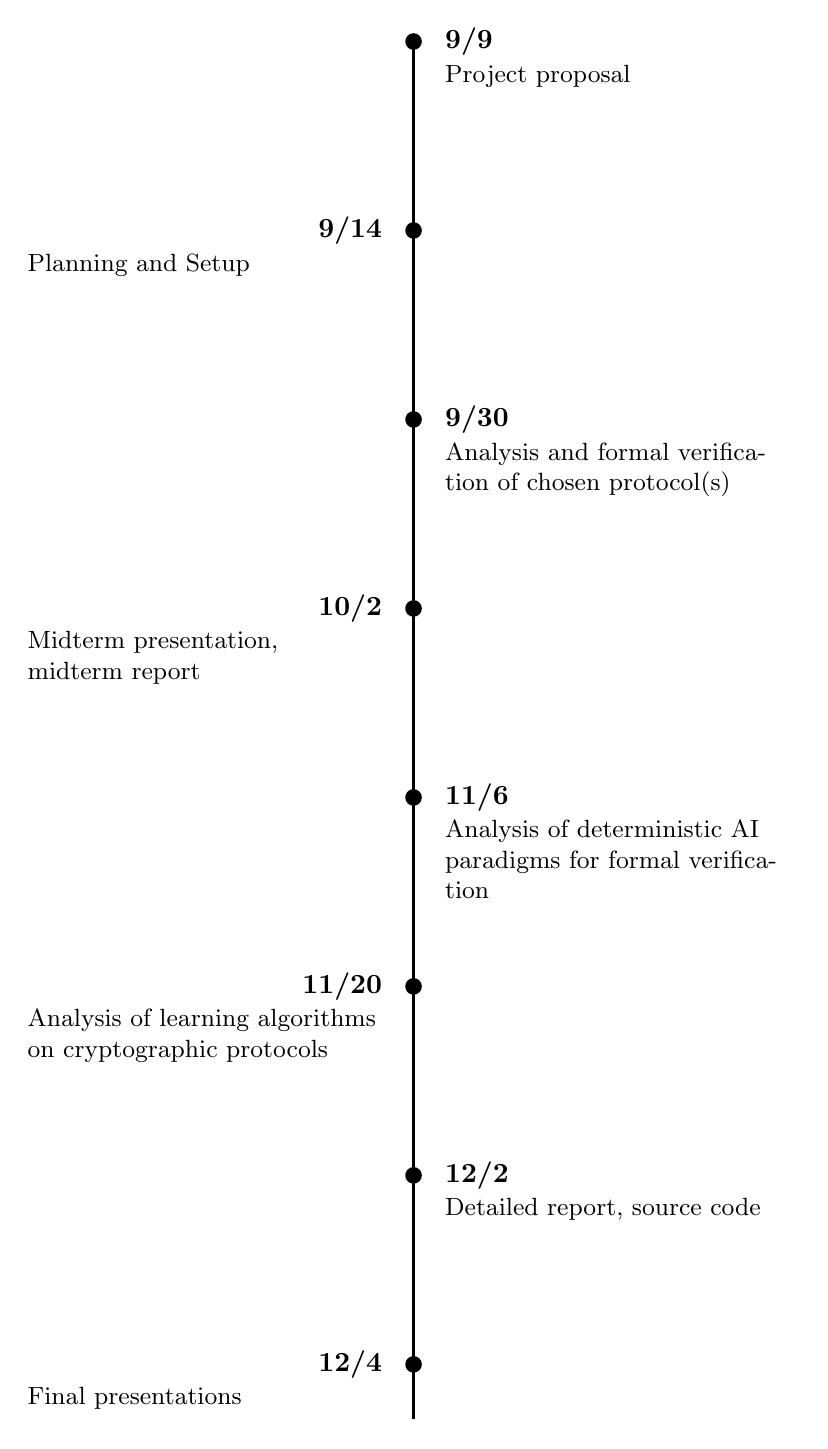
\begin{tikzpicture}[
    milestone/.style={circle, fill=black, minimum size=6pt, inner sep=0pt},
    datetext/.style={font=\bfseries, inner sep=0pt},
    desctext/.style={font=\small, align=left, text width=4.5cm, inner sep=0pt}
]
    % vertical line
    \draw[thick] (0,0) -- (0,-17.5);

    % milestone coordinates (top to bottom), evenly spaced
    \foreach \i/\y in {1/0, 2/-2.4, 3/-4.8, 4/-7.2, 5/-9.6, 6/-12, 7/-14.4, 8/-16.8}
        \node[milestone] (m\i) at (0,\y) {};

    % right-side entries (odd): description anchored a fixed gap below its own date
    \node[datetext, right=8pt of m1, anchor=west] (d1) {9/9};
    \node[desctext, below=3pt of d1.south west, anchor=north west] {Project proposal};

    \node[datetext, right=8pt of m3, anchor=west] (d3) {9/30};
    \node[desctext, below=3pt of d3.south west, anchor=north west] {Analysis and formal verification of chosen protocol(s)};

    \node[datetext, right=8pt of m5, anchor=west] (d5) {11/6};
    \node[desctext, below=3pt of d5.south west, anchor=north west] {Analysis of deterministic AI paradigms for formal verification};

    \node[datetext, right=8pt of m7, anchor=west] (d7) {12/2};
    \node[desctext, below=3pt of d7.south west, anchor=north west] {Detailed report, source code};

    % left-side entries (even): description anchored a fixed gap below its own date
    \node[datetext, left=8pt of m2, anchor=east] (d2) {9/14};
    \node[desctext, below=3pt of d2.south east, anchor=north east] {Planning and Setup};

    \node[datetext, left=8pt of m4, anchor=east] (d4) {10/2};
    \node[desctext, below=3pt of d4.south east, anchor=north east] {Midterm presentation, midterm report};

    \node[datetext, left=8pt of m6, anchor=east] (d6) {11/20};
    \node[desctext, below=3pt of d6.south east, anchor=north east] {Analysis of learning algorithms on cryptographic protocols};

    \node[datetext, left=8pt of m8, anchor=east] (d8) {12/4};
    \node[desctext, below=3pt of d8.south east, anchor=north east] {Final presentations};

\end{tikzpicture}
\caption{Project Timeline}
\end{figure}
\newpage

\subsection{Resources Required / Budget}
We have examined the resources required for this project in a previous section, ~\ref{sec:estprojbudget}. We see this information in budget chart form below.

\begin{center}
\small
\begin{tabular}{|l|l|l|l|}
\hline
\textbf{Item} & \textbf{Temporal Cost (hrs)} & \textbf{Monetary Cost} & \textbf{Mandatory (T/F)} \\
\hline
Team Research and Development & $520$ & \$0 & T \\
Faculty Sponsor Consultation Time  & 13 & \$0 & T \\
Problem Mentor Consultation Time & 13 & \$0 & T  \\
Extracurricular Research Hours & 520\footnotemark & \$0 & T  \\
\hline
\textbf{Total} & 546\footnotemark & \textbf{\$0} & N/A \\
\hline
\end{tabular}
\end{center}
\footnotetext{Subject to individual students, may not apply to all}
\footnotetext{Excluding Extracurricular Research Hours}


\section{Deliverables}
Several materials and artifacts will be created throughout the duration of the project. The main artifact consists of a detailed project report that describes the investigation and the results produced by the proposed project. Additional artifacts will either support the research being conducted or one of the two presentations for the program.

\begin{enumerate}
    \item \textbf{Project Bid}
    \begin{itemize}
        \item Due: 8/26/2026
        \item Bids expressing interests and approaches for 3 possible projects.
    \end{itemize}
    \item \textbf{Project Proposal}
    \begin{itemize}
        \item Date: 9/9/2026
        \item Detailed proposal explaining the scope of the project, motivations and significance. 
    \end{itemize}
    \item \textbf{Midterm Presentation}
    \begin{itemize}
        \item Date: c. 10/2/2026
        \item A midterm presentation summarizing the approach and current progress.
    \end{itemize}
    \item \textbf{Midterm Report}
    \begin{itemize}
        \item Date: c. 10/2/2025
        \item An interim report with more detailed research and project findings. 
    \end{itemize}
    \item \textbf{Detailed project report}
    \begin{itemize}
        \item Date: c. 12/2/2026
        \item A comprehensive report cataloging the project findings. The report will cover all 3 prongs of the project: an analysis and formal verification of a cryptographic protocol, the utility of a deterministic AI paradigm for formal verification, and whether a learning algorithm can successfully learn a protocol and expose existing or new vulnerabilities. 
    \end{itemize}
    \item \textbf{Source Code}
    \begin{itemize}
        \item Date: c. 12/2/2026
        \item Any code or scripts created in the process of implementing sections of the project.
    \end{itemize}
    \item \textbf{Final Presentation}
    \begin{itemize}
        \item Date: c. 12/4/2026
        \item A final presentation summarizing the project.
    \end{itemize}
\end{enumerate}

\section{Anticipated Challenges}
As of late, the field of protocol analysis and verification has advanced and many the publications thereof are self-contained. Since this project involves the research and application of certain tools, in particular constraint-based answer set programming languages such as s(CASP), previously not seen in Cybersecurity, this uncharted territory presents a unique opportunity for research, which in itself means a learning curve is to be expected for those team members who are not \text{ } experienced in research. Furthermore, since the nascent nature of this proposal leads Team Leader William to believe that deviations and revisions to the project's trajectory are to be expected (and welcomed). 

\section{Broader Impact}
Section~\ref{sec:mot} lays to bare the clear broader implications of our work. Recent attention on the analysis and verification of cryptographic protocols, in tandem with great interest in the utility of AI therein, compels us to our ultimate goal of seeing to fruition a new direction of research in the study of such protocols. Particularly, our novel use of goal-directed answer set programming presents a potentially fruitful use of the language in a new domain as well as an intrgiuing study into alternative forms of AI beyond the use of LLMs. 


\section{Investigator Bios}
\textbf{William T. Doan} is a Ph.D. in Computer Science student researching problems in data compression, compact data structures, and computational biology. Currently, one of his interests is in algorithmic techniques for differential privacy, in information theory, and algorithmic bound proving. William has considerable experience in AWS, software development, and agentic workflow orchestration through his internship. His coursework, and performance therein, demonstrates a strong proficiency in Computer Architecture, Database Systems (in which he has a paper publication forthcoming on using databases in deep learning), Computer Algorithms, Artificial Intelligence, Multicore Programming, Optimization, and Parallel Computing. Complementary to his rigorous academic portfolio is his research profile, wherein he is twice published in the conferences of the American Institute of Aeronautics and Astronautics for formal methods and certification, in IEEE’s Transactions on Multimedia for computer vision, in the Conference on Language Modeling for his deepfake research, in the Symposium on String Processing and Information Retrieval Conference for representing data compression as folding problems, and a forthcoming journal publication in optimizing DNA reconstruction. William has substantial experience leading research teams on the cutting-edge of research. Thus, he is highly interested in serving as the team leader for this project.\\

\noindent
\textbf{Aendri Singh} is pursuing a Master’s in Computer Science with a focus in Cybersecurity. She is interested in understanding how formal verification can be applied towards cryptographic protocols. Her coursework has involved computer networks \& security, Machine Learning, and information security. Through a previous internship, she conducted market research for non-human identity management and became a PingOne certified professional. She has previous experience leading a team of interns for a capstone project and currently works part-time as a computer science student mentor, covering topics related to discrete math and C/Java programming. She is currently taking an introductory cryptography course. Her coursework and experience with computer networks and AI leads her to want to understand how protocols are designed and implemented for AI communication and how they can be further modified or refined to increase security.\\

\noindent
\textbf{Pooya Zolfagharkhani} is a Computer Engineering master’s student and a full-time software design/development engineer. At work, he works on developing C/C++ software for real-time and mission-critical systems. His research and work experiences have allowed him to be familiar with software verification, evaluating generated code, and different approaches to best use LLMs. He is
interested in contributing to this project based on his experiences collaborating across engineering teams, performing code reviews, creating tasks for a project, and presenting technical details.\\

\noindent
\textbf{Andrew Bourinski} is a Computer Science master's student with a concentration in Cybersecurity. He has experience developing automation software in Python and establishing virtual environments to test and validate network configurations. His academic coursework in Automata Theory, Discrete Mathematics, and Computer Networks, alongside his CompTIA Security+ certification, provides a strong theoretical foundation in formal logic and cryptographic concepts. He also has experience managing technical projects, independently researching system capabilities, and validating approaches through structured testing. Based on his academic background and programming experience, he is well-prepared to model cryptographic specifications and evaluate protocols for this research effort.

\newpage
\section{Bibliography}
\renewcommand{\refname}{}
\vspace{-2.5em}
\bibliographystyle{unsrt}
\bibliography{bib}

%\newpage
%\section{Appendix A}
%\textbf{Acronyms}
%\begin{itemize}[noitemsep]
%    \item LI - Lorem Ipsum
%    \item LI-DSA - Lorem Ipsum Dolor Sit Amet
%\end{itemize}

\end{document}
